\documentclass[11pt]{article}

% ==== PACKAGES ==== %
% \usepackage{fullpage}
\usepackage{amsmath,amssymb,amsthm}
\usepackage{epic}
\usepackage{eepic}
\usepackage{hyperref}
\usepackage{listings}
\usepackage{float}
\usepackage{graphicx}
\usepackage{subcaption}
\usepackage{fancyhdr}
\usepackage{color}
\usepackage{bbm}
\usepackage[letterpaper, margin=1in]{geometry}

% ==== MARGINS ==== %
% \pagestyle{empty}
% \setlength{\oddsidemargin}{0in}
% \setlength{\textwidth}{6.8in}
% \setlength{\textheight}{9.5in}

\pagestyle{fancy}
\fancyhf{}
\rhead{ASEN 5044}
\lhead{Homework 1}
\rfoot{Page \thepage}


\newtheorem*{solution*}{Solution}
\newtheorem{lemma}{Lemma}[section]
\newtheorem{theorem}[lemma]{Theorem}
\newtheorem{claim}[lemma]{Claim}
\newtheorem{definition}[lemma]{Definition}
\newtheorem{corollary}[lemma]{Corollary}
\lstset{moredelim=[is][\bfseries]{[*}{*]}}

% ==== DOCUMENT PROPER ==== %
\begin{document}

\thispagestyle{empty}

% --- Header Box --- %
\newlength{\boxlength}\setlength{\boxlength}{\textwidth}
\addtolength{\boxlength}{-4mm}

\begin{center}\framebox{\parbox{\boxlength}{\bf
      Statistical Estimation \hfill Homework 2\\
      ASEN 5044 Fall 2018 \hfill Due Date: Sep 20, 2018\\
      Name: Andrew Kramer \hfill PhD Student
}}
\end{center}

\section*{Exercise 1}
Consider the equations of motion for a unit mass subjected to an inverse square law fore field,
\begin{align*}
	\ddot{r} &= r \dot{\theta}^2 + \frac{k}{r^2} + u_1(t) \\
	\ddot{\theta} &= -\frac{2\dot{\theta}\dot{r}}{r} + \frac{1}{r}u_2(t)
\end{align*}
where $r$ represents the radius from the center of the force field, $\theta$ gives the angle with respect to a reference direction in the orbital plane, $k$ is a constant, and $u_1$ and $u_2$ represent radial and tanjectial thrusts, respectively. It is easily shown that for the initial conditions $r(0) = r_0$, $\theta(0) = 0$, $\dot{r}(0) = 0$, and $\dot{\theta}(0) = \omega_0$ with nominal thrusts $u_1(t) = 0$ and $u_2(t) = 0$ for all $t \geq 0$ the equations of motion have as a solution the circular orbit given by
\begin{align*}
	r(t) &= r_0 = \text{constant} \\
	\dot{\theta}(t) &= \omega_0 = \text{constant} = \sqrt{\frac{k}{r_0^3}} \\
	\theta{t} &= \omega_0t + \text{constant}
\end{align*}
\subsection*{Problem (a)}
Pick a state vector for this system and express the original nonlinear ODEs in standard nonlinear state space form.

\subparagraph*{}
If we choose $x = [r,\ \theta, \dot{r}, \dot{\theta}]^T$ as our state vector and $y = [r,\ \theta]^T$ as our observation vector then we can express the original ODEs as
\begin{align*}
	\dot{x} &= \begin{bmatrix} \dot{x_1} \\ \dot{x_2} \\ \dot{x_3} \\ \dot{x_4} \end{bmatrix} 
	= \begin{bmatrix} x_3 \\
				x_4 \\
				x_1x_4^2 - \frac{k}{x_1^2}+u_1(t) \\
				-\frac{2x_4x_3}{x_1} + \frac{1}{x_1}u_2(t)
				\end{bmatrix} \\
	y &= \begin{bmatrix} x_1 \\ x_2 \end{bmatrix}
\end{align*}

\subsection*{Problem (b)}
Linearize this system's nominal equations of motion about the nominal solution $r(t) = r_0$, $\dot{r}(0) = 0$, $\theta(t) = \omega_0t+\text{constant}$ and $\dot{\theta}(t) = \omega_0$ with $u_1(t) = 0$ and $u_2(t) = 0$. Find $(A,B,C,D)$ matrices for output $y(t)=[r(t),\theta(t)]^T$ for the linearized system of equations about the nominal solution.

\subparagraph*{}
If we take $x_\text{nom} = [r_0,0,\omega_0t+c,\omega_0]^T$ and $u_\text{nom} = [0,0]^T$. We can say $x(t)=x_\text{nom}(t)+\tilde{x}(t)$ and $u(t) = u_\text{nom}(t) + \tilde{u}(t)$. We can define 
\begin{align*}
	\dot{\tilde{x}} &= A_\text{nom} \tilde{x}(t) + B_\text{nom}\tilde{u}(t) \\
	A_\text{nom} = \left. \frac{\partial f}{\partial x} \right|_{x_\text{nom},u_\text{nom}} &= \begin{bmatrix} 0 & 0 & 1 & 0 \\
	0 & 0 & 0 & 1 \\ \omega_0^2+2\frac{k}{r_0^3} & 0 & 0 & 2r_0\omega_0 \\ 0 & 0 & -\frac{2\omega_0}{r_0} & 0 \end{bmatrix} \\
	B_\text{nom} = \left. \frac{\partial f}{\partial u} \right|_{x_\text{nom},u_\text{nom}} & = \begin{bmatrix} 0 & 0 \\ 0 & 0 \\ 1 & 0 \\ 0 & \frac{1}{r_0} \end{bmatrix}
\end{align*}
The observation function is already linear, so the $C$ and $D$ matrices do not need to be linearized:
\begin{align*}
	y(t) &= Cx(t) + Du(t) \\
	C &= \begin{bmatrix} 1 & 0 & 0 & 0 \\ 0 & 1 & 0 & 0 \end{bmatrix} \\
	D &= \begin{bmatrix} 0 & 0 \\ 0 & 0 \end{bmatrix}
\end{align*}

\subsection*{Problem (c)}
Convert the continuous time $(A,B,C,D)$ matrices you found from part (b) into discrete time $(F,G,H,M)$ matrices using a discretization step size of $\Delta t=10\text{s}$ and setting $k=398600\text{km}^3/\text{s}^2$ and $r_0=6678$km.

\subparagraph*{}
We start by reorganizing our ODE as $\dot{\tilde{x}}_a = \hat{A}[\tilde{x}, \tilde{u}]^T$ where
\begin{equation*}
	\hat{A} = \begin{bmatrix} A & B \\ 0 & 0 \end{bmatrix} = \begin{bmatrix} 0 & 0 & 1 & 0 & 0 & 0 \\ 0 & 0 & 0 & 1 & 0 & 0 \\ \omega_0^2 + 2\frac{k}{r_0^3} & 0 & 0 & 2r_0\omega_0 & 1 & 0 \\ 0 & 0 & -\frac{2\omega_0}{r_0} & 0 & 0 & \frac{1}{r_0} \\ 0 & 0 & 0 & 0 & 0 & 0 \\ 0 & 0 & 0 & 0 & 0 & 0 \end{bmatrix} = \begin{bmatrix} 0 & 0 & 1 & 0 & 0 & 0 \\ 0 & 0 & 0 & 1 & 0 & 0 \\ 0.00157 & 0 & 0 & 0.01788 & 1 & 0 \\ 0 & 0 & 4.01\times10^{-10} & 0 & 0 & 1.497\times10^{-4} \\ 0 & 0 & 0 & 0 & 0 & 0 \\ 0 & 0 & 0 & 0 & 0 & 0 \end{bmatrix}
\end{equation*}
We know that $F$ will be the upper left $n\times n$ submatrix and $G$ will be the the upper right $m\times n$ submatrix of $e^{\hat{A}\Delta t}$:
\begin{align*}
	e^{\hat{A}\Delta t} &= \begin{bmatrix} 1.079 & 0 & 10.26 & 0.906 & 50.65 & 4.496\times10^{-4} \\ 0 & 1 & 0 & 10 & 0 & 7.485\times10^{-3} \\ 0.0161 & 0 & 1.079 & 0.184 & 10.264 & 1.35\times10^{-4} \\ 0 & 0 & 0 & 1 & 0 & 1.497\times10^{-3} \\ 0 & 0 & 0 & 0 & 1 & 0 \\ 0 & 0 & 0 & 0 & 0 & 1 \end{bmatrix} \\
	F &= \begin{bmatrix} 1.079 & 0 & 10.26 & 0.906 \\ 0 & 1 & 0 & 10 \\ 0.0161 & 0 & 1.079 & 0.184\\ 0 & 0 & 0 & 1 \end{bmatrix} \\
	G &= \begin{bmatrix} 50.65 & 4.496\times10^{-4} \\ 0 & 7.485\times10^{-3} \\ 10.264 & 1.35\times10^{-4} \\ 0 & 1.497\times10^{-3} \end{bmatrix}
\end{align*}
The $H$ and $M$ matrices for the discretized system are simply equal to the $C$ and $D$ matrices for the continuous time system:
\begin{align*}
	H &= C \\
	M &= D
\end{align*}

\subsection*{Problem (d)}
Interpret the results for the STM in part (c), i.e. what is the physical meaning of each column vector that makes up $F$?

\subparagraph{}
Each column vector $F_i$ in $F$ represents how $\tilde{x}_i(k)$ contributes to $\tilde{x}(k+1)$. In other words, each column vector describes how the corresponding entry in the $\tilde{x}$ vector at step $k$ will affect the entire $\tilde{x}$ vector at step $k+1$.

\section*{Exercise 2}
The linear position $p$ of an object under constant acceleration is
\begin{equation*}
	p = p_0 + \dot{p}_0t + \frac{1}{2}\ddot{p}_0t^2
\end{equation*}
where $p_0$ is the initial position of the object.

\subsection*{Problem (a)}
Define a state vector as $x=[p\ \dot{p}\ \ddot{p}]^T$ and write the state space equation $\dot{x} = Ax$ for this system.

\subparagraph*{}
Because the object is under constant acceleration, the derivative of the acceleration $\dddot{p} = 0$. So the state space equation is simply:
\begin{equation*}
	\begin{bmatrix} \dot{p} \\ \ddot{p} \\ \dddot{p} \end{bmatrix} = \begin{bmatrix} 0 & 1 & 0 \\ 0 & 0 & 1 \\ 0 & 0 & 0 \end{bmatrix} \begin{bmatrix} p \\ \dot{p} \\ \ddot{p} \end{bmatrix}
\end{equation*}

\subsection*{Problem (b)}
Use the first and last expressions in Equation (1.71) to find the state transition matrix for this system.

\subparagraph*{}
We'll first go through the infinite series method, calculating the powers of $A$ first:
\begin{align*}
	A\Delta t &= \begin{bmatrix} 0 & \Delta t & 0 \\
								 0 & 0 & \Delta t \\
								 0 & 0 & 0 \end{bmatrix} \\
	(A\Delta t)^2 &= \begin{bmatrix} 0 & 0 & \Delta t^2 \\
									 0 & 0 & 0 \\
									 0 & 0 & 0 \end{bmatrix} \\
	(A\Delta t)^3 &= \begin{bmatrix} 0 & 0 & 0 \\
									 0 & 0 & 0 \\
									 0 & 0 & 0 \end{bmatrix}
\end{align*}
Luckily for us, $(A\Delta t)^3$ is the zero matrix, so we don't have to extend the series beyond $i=2$. This means the state transition matrix can be calculated as follows:
\begin{align*}
	e^{A\Delta t} &= \sum_{i=0}^2 \frac{(A\Delta t)^i}{i!} \\
	&= I + \begin{bmatrix} 0 & \Delta t & 0 \\
						   0 & 0 & \Delta t \\
						   0 & 0 & 0 \end{bmatrix} 
		+ \frac{1}{2} \begin{bmatrix} 0 & 0 & \Delta t^2 \\
									  0 & 0 & 0 \\
									  0 & 0 & 0 \end{bmatrix} \\
	&= \begin{bmatrix} 1 & \Delta t & \frac{1}{2}\Delta t^2 \\
					   0 & 1 & \Delta t \\
					   0 & 0 & 1 \end{bmatrix}
\end{align*}
When employing the third expression in equation 1.71, we find that $\hat{A} = A$ and $Q = I$. Since $\hat{A} = A$ we can't use the third expression to try to find $e^{\hat{A}\Delta t}$ as this would lead us into an infinite loop, so we'll use the result from above. Thus, the third expression gives
\begin{align*}
	e^{A\Delta t} &= Qe^{\hat{A}\Delta t}Q^{-1} \\
	&= \begin{bmatrix} 1 & 0 & 0 \\ 0 & 1 & 0 \\ 0 & 0 & 1 \end{bmatrix} \begin{bmatrix} 1 & \Delta t & \frac{1}{2} \Delta t^2 \\ 0 & 1 & \Delta t \\ 0 & 0 & 1 \end{bmatrix} \begin{bmatrix} 1 & 0 & 0 \\ 0 & 1 & 0 \\ 0 & 0 & 1 \end{bmatrix}^{-1} \\
	&= \begin{bmatrix} 1 & \Delta t & \frac{1}{2}\Delta t^2 \\
					   0 & 1 & \Delta t \\
					   0 & 0 & 1 \end{bmatrix}
\end{align*}

\subsection*{Problem (c)}
Prove for the state transition matrix found above that $e^{A0} = I$.

\subparagraph*{} 
\begin{equation*}
	e^{A0} = \begin{bmatrix} 1 & 0 & 0^2 \\
							 0 & 1 & 0 \\
							 0 & 0 & 1 \end{bmatrix}
			= \begin{bmatrix} 1 & 0 & 0 \\
							  0 & 1 & 0 \\
							  0 & 0 & 1 \end{bmatrix}
\end{equation*}

\section*{Exercise 3}
Consider the following system matrix
\begin{equation*}
	A = \begin{bmatrix} 1 & 0 \\ 0 & -1 \end{bmatrix}
\end{equation*}
Show that the matrix
\begin{equation*}
	S(t) = \begin{bmatrix} e^t & 0 \\ 0 & 2e^{-t} \end{bmatrix}
\end{equation*}
satisfies the relation $\dot{S}(t) = AS(t)$, but $S(t)$ is not the state transition matrix of the system.

\subparagraph*{}
First we find the state transition matrix of the system:
\begin{align*}
	e^{At} &= \sum_{i=0}^\infty \frac{(At)^i}{i!} \\
	&= I + \begin{bmatrix} t & 0 \\ 0 & -t \end{bmatrix} + \frac{1}{2!} \begin{bmatrix} t^2 & 0 \\ 0 & t^2 \end{bmatrix} + \frac{1}{3!} \begin{bmatrix} t^3 & 0 \\ 0 & -t^3 \end{bmatrix} + \dots \\
	&= \begin{bmatrix} \sum_{j=0}^\infty \frac{t^j}{j!} & 0 \\ 0 & \sum_{j=0}^\infty (-1)^j\frac{t^j}{j!} \end{bmatrix} \\
	&= \begin{bmatrix} e^t & 0 \\ 0 & e^{-t} \end{bmatrix}
\end{align*}
It is clear that $e^{At} \neq S(t)$. Now we can show that $\dot{S}(t) = AS(t)$. 
\begin{align*}
	\dot{S}(t) &= \begin{bmatrix} \frac{\partial}{\partial t} e^t & 0 \\ 0 & \frac{\partial}{\partial t} 2e^{-t} \end{bmatrix} = \begin{bmatrix} e^t & 0 \\ 0 & -2e^{-t} \end{bmatrix} \\
	AS(t) &= \begin{bmatrix} 1 & 0 \\ 0 & -1 \end{bmatrix} \begin{bmatrix} e^t & 0 \\ 0 & 2e^{-t} \end{bmatrix} = \begin{bmatrix} e^t & 0 \\ 0 & -2e^{-t} \end{bmatrix}
\end{align*}

\section*{Exercise 4}
The vertical dimension of a hovering rocket can be modeled as
\begin{align*}
	\dot{x}_1 &= x_2 \\
	\dot{x}_2 &= \frac{Ku-gx_2}{x_3} - \frac{GM}{(R+x_1)^2} \\
	\dot{x}_3 &= -u
\end{align*}
where $x_1$ is the vertical position of the rocket, $x_2$ is the vertical velocity, $x_3$ is the mass of the rocket, $u$ is the control input (the flow rate of rocket propulsion), $K=1000$ is the thrust constant, $g=50$ is the drag constant, $G=6.673\times10^{-11}\frac{\text{m}^3}{\text{kg}/\text{s}^2}$ is the gravitational constant, $M=5.98\times10^{24}\text{kg}$ is the mass of earth, and $R=6.37\times10^6\text{m}$ is the radius of the earth.

\subsection*{Problem (a)}
Find $u(t)=u_0(t)$ such that the system is in equilibrium at $x_1(t)=0$ and $x_2(t)=0$.

\subparagraph*{}
If the system is in equilibrium the rocket is stationary at some altitude $x_{1,0}$, so $\dot{x}_1 = \dot{x}_2 = 0$. So from the given equations we can say
\begin{align*}
	\dot{x}_1 &= x_2 = 0 \\
	\dot{x}_2 &= \frac{Ku}{x_3} - \frac{GM}{R^2} = 0\\
	\frac{Ku}{x_3} &= \frac{GM}{R^2} \\
	u_0(t) &= \frac{GMx_3(t)}{KR^2}
\end{align*}
We can interpret this result physically as follows: the rocket's thrust must be equal to the gravitational force between the earth and the rocket. This agrees with Newton's laws, so we can be fairly confident we're on the right track. 

\subsection*{Problem (b)}
Find $x_3(t)$ when $x_1(t)=0$ and $x_2(t)=0$.

\subparagraph*{}
$x_3$ is simply the integral of $-u(t)$:
\begin{equation*}
	x_3(t) = -\int_{0}^{t}u(t)dt
\end{equation*}
However, we also know from part (a) that $x_3(t) =  \frac{KR^2}{GM}u_0(t)$. This means $u_0(t)$ is governed by the differential equation
\begin{align*}
	\frac{KR^2}{GM}u_0(t) &= -\int_0^t u(t)dt\\
	u_0(t) &= -\frac{GM}{KR^2}\int_0^tu_0(t) \\
	\frac{d}{dt}u_0(t) = -\frac{GM}{KR^2}u_0(t) \\
	u_0(t) &= e^{-(GM/KR^2)t}
\end{align*}
So the nominal value for $x_3(t)$ is
\begin{equation*}
	x_3(t) = -\int_{0}^{t}u(t)dt = \left. \frac{KR^2}{GM} e^{-(GM/KR^2)t} \right |_{0,t} + \text{const.}
\end{equation*}
We can take the constant to be $x_\text{dry}$, the dry (unfueled) mass of the rocket. This means the coefficient on the exponential must be equal to the mass of the fuel on the rocket (i.e. the initial mass of the rocket minus the dry mass) so the expression for $x_3(t)$ can be simplified to
\begin{equation*}
	x_3(t) = (x_{3,0} - x_\text{dry})e^{-(GM/KR^2)t} + x_\text{dry}
\end{equation*}

\subsection*{Problem (c)}
Linearize the system around the state trajectory found above.

\subparagraph*{}
We first define
\begin{equation*}
	\dot{x} = f(x,u,t) = \begin{bmatrix} x_2 \\ \frac{Ku-gx_2}{x_3} - \frac{GM}{(R+x_1)^2} \\ -u \end{bmatrix}
\end{equation*}
From this we can find the jacobians of $f$ with respect to $x$ and $u$.
\begin{align*}
	\frac{\partial f}{\partial x} &= \begin{bmatrix} 0 & 1 & 0 \\ 2\frac{GM}{(R+x_1)^3} & \frac{-g}{x_3} & -\frac{Ku-gx_2}{x_3^2} \\ 0 & 0 & 0 \end{bmatrix} \\
	\frac{\partial f}{\partial u} &= \begin{bmatrix} 0 \\ \frac{K}{x_3} \\ -1 \end{bmatrix}
\end{align*}
We then evaluate the jacobians at $x_{\text{nom}} = [0,\ 0,\ \frac{KR^2}{GM}e^{-(GM/KR^2)t} + x_{3,0}]^T$, $u_{\text{nom}}=e^{-(GM/KR^2)t}$ to find the $A_\text{nom}$ and $B_\text{nom}$ matrices of the linearized system. We'll also define $\frac{GM}{KR^2} = \alpha$ so that $x_{3,\text{nom}} = (x_{3,0}-x_\text{dry})e^{-\alpha t} + x_\text{dry}$ and $u_\text{nom} = e^{-\alpha t}$. 
\begin{align*}
	A_\text{nom} &= \left. \frac{\partial f}{\partial x} \right |_{x_{\text{nom}},u_{\text{nom}}} = \begin{bmatrix} 0 & 1 & 0 \\ \frac{2GM}{R^3} & -\frac{g}{(x_{3,0}-x_\text{dry})e^{-\alpha t} + x_\text{dry}} & -\frac{-\alpha Ke^{-\alpha t}}{((x_{3,0}-x_\text{dry})e^{-\alpha t} + x_\text{dry})^2} \\ 0 & 0 & 0 \end{bmatrix} \\
	B_\text{nom} &= \left. \frac{\partial f}{\partial u} \right |_{x_{\text{nom}},u_{\text{nom}}} = \begin{bmatrix} 0 \\ \frac{K}{(x_{3,0}-x_\text{dry})e^{-\alpha t} + x_\text{dry}} \\ -1 \end{bmatrix}
\end{align*}

\subsection*{Problem (d)}
Simulate the nonlinear system for five seconds (using MATLAB's \texttt{ode45} command) and the linearized system for five seconds with $u(t)=u_0(t)+\Delta u\text{ abs}(\cos(t))$ and $x_{3,0}=1000\text{kg}$. Plot the altitude of the rocket for both simulations on the same plot when $\Delta u=10$. Repeat for $\Delta u=100$ and $\Delta u=300$. Hand in your source code and the three plots. What can you conclude about the accuracy of your linearization?

\subparagraph*{}
See below for the Matlab code used to model the given system. \texttt{nonLinear.m} defines the function to model the nonlinear system, \texttt{linearized.m} defines the function to model the linearized system, and \texttt{runODE.m} sets up and runs the ODE and plots the results.

\lstinputlisting[language=Matlab, caption=nonLinear.m]{nonLinear.m}
\lstinputlisting[language=Matlab, caption=linearized.m]{linearized.m}
\lstinputlisting[language=Matlab, caption=runODE.m]{runODE.m}

On figure \ref{fig:10}, below, we can see that for small perturbations in $\Delta u$, the linearized model follows the linear model very closely. When $\Delta u=100$, as in figure \ref{fig:100}, we can see that the linearized model differs from the nonlinear model more than when $\Delta u = 10$, but the shape of the linearized function still tracks the nonlinear model very closely. Lastly, in plot \ref{fig:300} when $\Delta u=300$ we can see that the linearized function diverges significantly from the nonlinear. From this we can see that the linearized model is only valid for relatively small perturbations from the nominal values for state and input.

\begin{figure}[h!]
	\centering
	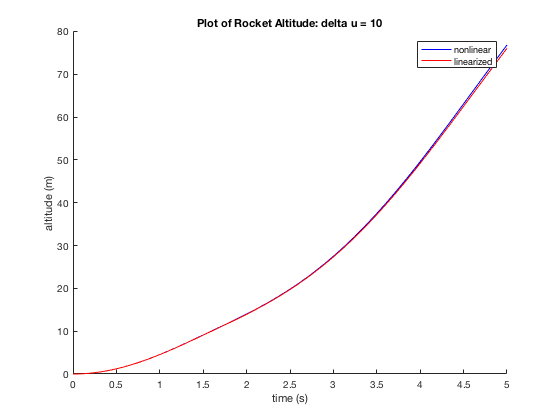
\includegraphics[width=0.6\linewidth]{plot10.png}
	\caption{}
	\label{fig:10}
\end{figure}

\begin{figure}[h!]
	\centering
	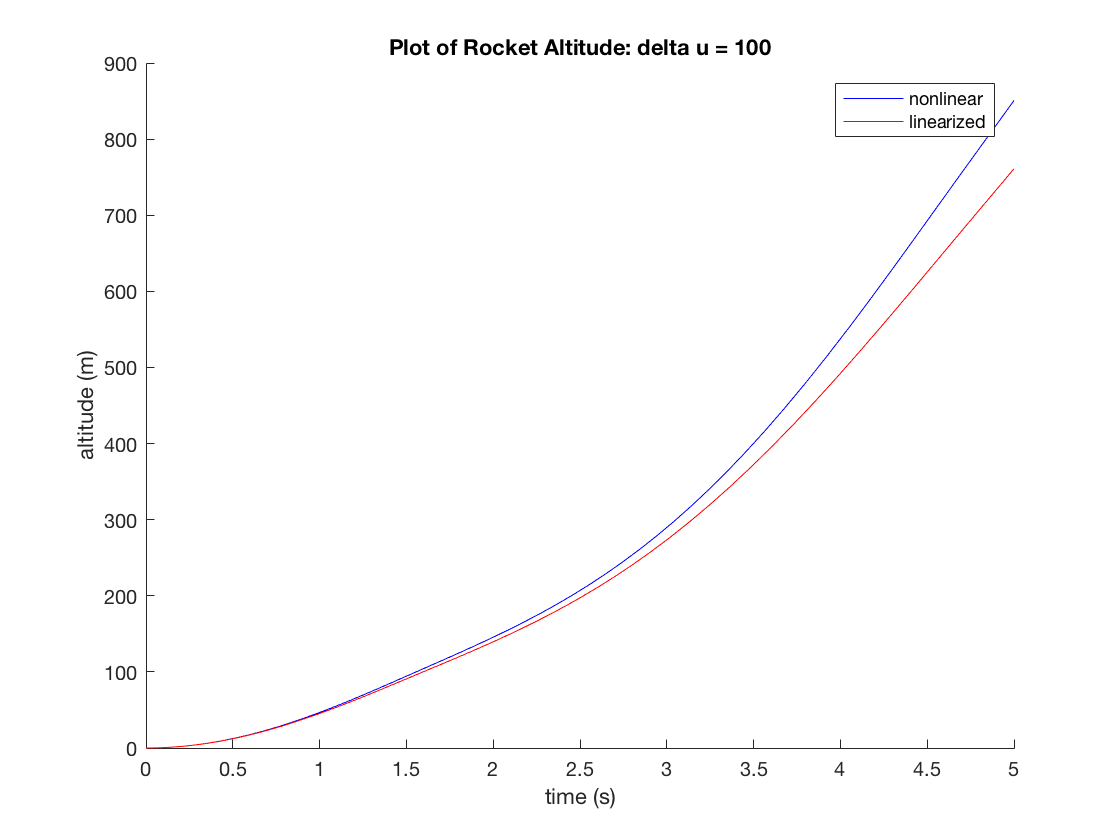
\includegraphics[width=0.6\linewidth]{plot100.png}
	\caption{}
	\label{fig:100}
\end{figure}
\begin{figure}[h!]
	\centering
	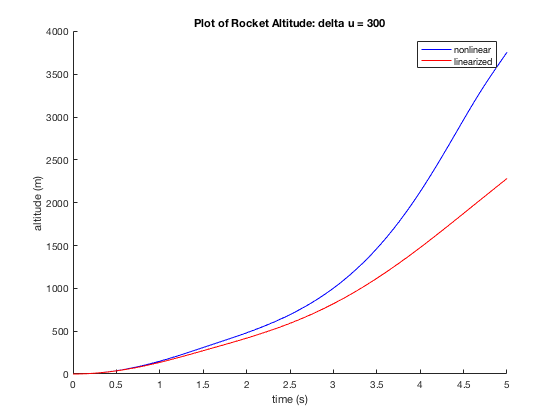
\includegraphics[width=0.6\linewidth]{plot300.png}
	\caption{}
	\label{fig:300}
\end{figure}

\section*{Exercise A1}
Suppose $A$ is invertible and 
\begin{equation*}
	\begin{bmatrix} A & A \\ B & A \end{bmatrix} \begin{bmatrix} A \\ C \end{bmatrix} = \begin{bmatrix} 0 \\ I \end{bmatrix}
\end{equation*}
Find $B$ and $C$ in terms of $A$.

\subparagraph*{}
The expression above reduces to the following:
\begin{align*}
	A^2 + AC &= 0 \\
	C &= A^{-1}(-A^2) \\
	&= -A \\
	BA + AC &= I \\
	BA - AA^{-1}A^2 &= I \\
	BA &= I + A^2 \\
	B &= A^{-1}(I+A^2) \\
	&= A^{-1} + A
\end{align*}

\section*{Exercise A2}
Show that $|e^{At}|=e^{\text{tr}(A)t}$ for any square matrix $A$.

\subparagraph*{}
Let's first assume that $A$ is diagonal. In this case the exponential of $A$ is a diagonal matrix $\Lambda$ where the diagonal elements $\lambda_{ij} = e^{a_{ij}}$. This means that
\begin{align*}
	det{e^{At}} &= e^{a_{1,1}t} \times \dots \times e^{a_{n,n}t} \\
	&= e^{(a_{1,1} + \dots + a_{n,n})t} \\
	&= e^{\text{tr}(A)t}
\end{align*}
Now let's assume that $A$ is diagonalizable. In this case there exists a matrix $B$ such that $P^{-1}\Lambda P = A$ where $\Lambda$ is the diagonalized form of $A$. We can show that because
\begin{align*}
	A^2 &= (P^{-1}\Lambda P)(P^{-1}\Lambda P) \\
	&= P^{-1}\Lambda (PP^{-1}) \Lambda P \\
	&= P^{-1} \Lambda P
\end{align*}
and higher powers follow the same pattern that
\begin{equation*}
	e^A = P^{-1}\Bigg[\sum_{i=0}^\infty \frac{\Lambda^i}{i!} \Bigg] P
\end{equation*}
So $e^At = P^{-1}e^{\Lambda t} P$. Also, since the determinant of the product of square matrices is the product of the determinants of those matrices,
\begin{align*}
	|e^{At}| &= |P^{-1}e^{\Lambda t}P| \\
	&= |P^{-1}||e^{\Lambda t}||P| \\
	&= |e^{\Lambda t}| \\
	&= e^{\text{tr}(\Lambda) t}
\end{align*}
So because $\text{tr}(\Lambda)=\text{tr}(A)$ this shows $|e^{At}|=e^{\text{tr}(A)t}$ when A is diagonalizable. Finally, for the general case we'll use the jordan form of $A$ where $QAQ^{-1}=J$ and $A=Q^{-1}JQ$. From our arguments in the previous case we can say that $e^A=Q^{-1}e^JQ$. Therefore
\begin{equation*}
	|e^{At}| = |Q^{-1}e^{Jt}Q|=|e^{Jt}|
\end{equation*}
Because $J$ is upper triangular and the determinant of an upper triangular matrix is the product of its diagonal elements, and the trace of $J$ is equal to the trace of $J$ we can say that $|e^{At}| = e^{\text{tr}(A)}$.

\end{document}
